% style setup
% -----------------------------------------------------------------------
\documentclass[10pt,landscape]{article}
\usepackage{amssymb,amsmath,amsthm,amsfonts}
\usepackage{amsmath}
\usepackage{amssymb}
\usepackage{multicol,multirow}
\usepackage[utf8]{inputenc}
\usepackage{calc}
\usepackage{ifthen}
\usepackage[landscape]{geometry}
\usepackage[colorlinks=true,citecolor=blue,linkcolor=blue]{hyperref}
\usepackage[colorlinks=true,citecolor=blue,linkcolor=blue]{hyperref}
\usepackage{graphicx}


\ifthenelse{\lengthtest { \paperwidth = 11in}}
    { \geometry{top=.5in,left=.5in,right=.5in,bottom=.5in} }
	{\ifthenelse{ \lengthtest{ \paperwidth = 297mm}}
		{\geometry{top=1cm,left=1cm,right=1cm,bottom=1cm} }
		{\geometry{top=1cm,left=1cm,right=1cm,bottom=1cm} }
	}
\pagestyle{empty}
\makeatletter
\renewcommand{\section}{\@startsection{section}{1}{0mm}%
                                {-1ex plus -.5ex minus -.2ex}%
                                {0.5ex plus .2ex}%x
                                {\normalfont\large\bfseries}}
\renewcommand{\subsection}{\@startsection{subsection}{2}{0mm}%
                                {-1explus -.5ex minus -.2ex}%
                                {0.5ex plus .2ex}%
                                {\normalfont\normalsize\bfseries}}
\renewcommand{\subsubsection}{\@startsection{subsubsection}{3}{0mm}%
                                {-1ex plus -.5ex minus -.2ex}%
                                {1ex plus .2ex}%
                                {\normalfont\small\bfseries}}
\makeatother
\setcounter{secnumdepth}{0}
\setlength{\parindent}{0pt}
\setlength{\parskip}{0pt plus 0.5ex}
% -----------------------------------------------------------------------
% -----------------------------------------------------------------------
% -----------------------------------------------------------------------

\title{Quick Guide to LaTeX}

\begin{document}

\footnotesize

% -----------------------------------------------------------------------
% -----------------------------------------------------------------------
% -----------------------------------------------------------------------



\begin{center}
     \Large{\textbf{Time Series Analysis}} \\
\end{center}



\section{What is time series}
A collection of stochastic random variables \textbf{indexed by time}, their stochastic \textbf{distributions are similar but not the same}, the data are \textbf{correlated across time}\\
In plain words, time series refers to \textbf{a series of data points}, for which they follow some kind of distribution.\\
\textbf{The goal for studying time series}, is really to investigate in those data points, and try to figure out its \textbf{underlying distribution, and internal correlation} 
\subsection{Important Characteristics}
\begin{enumerate}
	\item Trend
	\item Seasonality
	\item Periodicity
	\item Cyclical Trend
	\item Heteroskedasticity
	\item Dependence
\end{enumerate}

\subsection{Presentation \& Basic Decomposition}
$Y_t, \text{ in which t indexes time: }$ $Y_t = m_t+s_t+x_t$ $, with :$
$\\m_t \text{ --- trend component, trend means that over the time scope, the values are going up or going down}, 
\\s_t \text{ --- seasonal component, seasonality means that it is a periodicity movement, it has a circle of appearance, within the circle, the overall trend should be zero }. 
\\x_t \text{ --- stationary component, stationary means still, it pictures the characteristic that the component is not changing its value}$\\
	



\begin{multicols}{3}
\setlength{\premulticols}{1pt}
\setlength{\postmulticols}{1pt}
\setlength{\multicolsep}{1pt}
\setlength{\columnsep}{2pt}

	
\section{Estimate the trend}
\begin{enumerate}
	\item Moving Average: \\estimate the trend with a moving window
	\item Parametric Regression \\ fit in a polynomial regression to estimate
	\item Non-Parametric Approach
	\begin{itemize}
	\item Kernel Regression
	\item Local Polynomial Regression
	\item Other Approaches 
\end{itemize}

\texttt{
Example: Temperature Data\\
1. Read the data file in R\\
2. Visualize the data (Avg Temp)\\
3. Estimate the trend (Moving Average)\\
4. Estimate the trend (Parametric)\\
5. Estimate the trend (Non-Parametric)\\
6. Comparison
}

\end{enumerate}


\section{Estimate the Seaonality}
General Approach: estimate and subtract $m_t$ and $s_t$\\

\begin{enumerate}
	\item Seasonal Average
			\\ $\hat s_k = w_k - \frac{1}{d}\sum_{j=1}^d w_j$\\
			\\ $k$: the seasonal group, let's say it has d groups. If the seasonality is monthly, then d = 12
			\\ $w_k$: the average of all seasonal group value
			
	\item Parametric Regression

\texttt{
Example: Temperature Data\\
1. Read the data file in R\\
2. Visualize the data (Avg Temp)\\
3. Estimate the trend (Moving Average)\\
4. Estimate the trend (Parametric)\\
5. Estimate the trend (Non-Parametric)\\
6. Comparison
}

\end{enumerate}

\section{Estimate the Stationary}


\end{multicols}


\newpage
\begin{multicols}{3}
\setlength{\premulticols}{1pt}
\setlength{\postmulticols}{1pt}
\setlength{\multicolsep}{1pt}
\setlength{\columnsep}{2pt}



\section{Important Concepts in Time Series}
\begin{enumerate}
  \item \textbf{Auto Correlation Function (ACF)}\\
  		Like correlation or covariance, the auto correlation between 2 variables can be expressed as:\\
  		$
  		\gamma(s,t) = Cov(X_s, X_t) = E[(X_s - \mu_s)(X_t-\mu_t)]\\
  		\gamma(t,t) = Var[X_t] = \sigma^2\\
  		\text{then we have the auto correlation defined as:}\\
  		\gamma_k = \gamma(t, t+k) \approx c_k \rightarrow \frac{\sum(x_t - \bar x)(x_{t+k}-\bar x)}{N} \\
  		\text{}
  		$The underlying assumption is that the time series is stationary, therefore, across all k time horizon, this auto correlation relationship exist
  \item \textbf{Auto Correlation Coefficient}\\
  		Following the auto correlation, the auto correlation coefficient can be defined as:
  		$
  		\rho_K = \frac{\gamma_k}{\gamma_0} \approx r_k \rightarrow \frac{c_k}{c_0}
  		$
  		
  \item \textbf{Partial Auto Correlation Function (PACF)}\\
  		For a series of data\\
  		\textbf{We first start at a point and look backwards:}\\
  		$
  		\hat x_{t+h} = \beta_1 x_{t+h-1} + \beta_2 x_{t+h-2} + ... + \beta_{h-1} x_{t+1}\\
  		$
  		Note that  $\beta$  is how far away from target variables\\
  		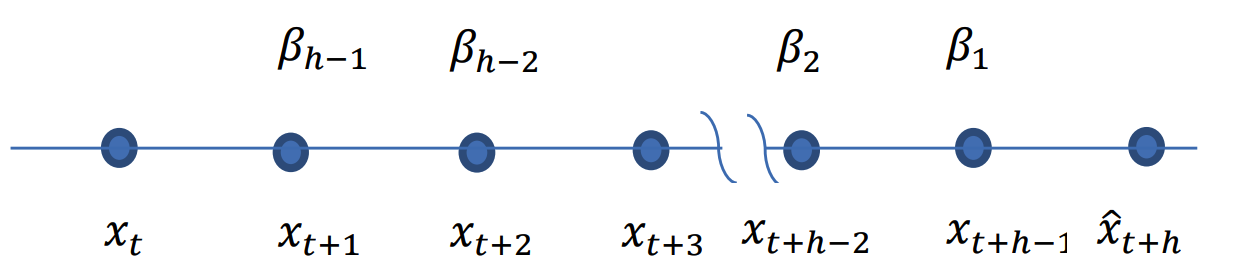
\includegraphics[width=60mm,scale=1]{images/PACF-1.png}
  		
  		\textbf{Then we try looking forwards:}\\
  		$
  		x_{t} = \beta_1 x_{t+1} + \beta_2 x_{t+2} + ... + \beta_{h-1} x_{t+h-1}\\
  		$
  		Note that  $\beta$  is how far away from target variables\\
  		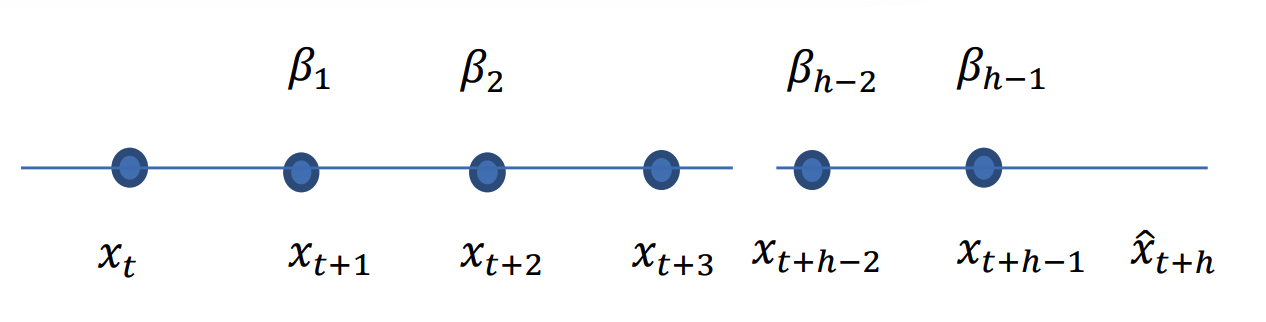
\includegraphics[width=60mm,scale=1]{images/PACF-2.png}
  		
  		\textbf{Finally we remove the predict and see residual:}\\
  		$
  		Corr[(x_{t+h}- \hat x_{t+h}), (x_t - \hat x_t)]
  		$\\
  		Therefore, this model measure the correlation with a lag, without accounting for the effect of variables in between.\\
  		
  		
  		Take away: Partial Out a variable, what PACF measures  		
  \item \textbf{Random Walk}\\
  		$
  		X_t = X_{t-1}+Z_t\\
  		\text{Z as the white noise, X as stock price}\\
  		X_t = \sum_{i=1}^t Z_i\\
  		\text{we can interpret X as accumulated white noise}\\
  		E[X_t] = \mu t \ , \ Var[X_t] = \sigma^2 t
  		$
  \item \textbf{Moving Average Process: q}\\
  		How long back need to trace, to have weighted average:\\
  		The longer we trace back, distribution be smoother:\\
  		$
  		\text{For instance, the MA(2) process is correlated back in 2 steps:}\\
  		X_t = Z_t + \theta_1 Z_{t-1} + \theta_2 Z{t-2}\\
  		Z_t \sim N(0,1)
  		$
  		
  		Moving Average is Weakly Stationary:
  		
  		$
  		cov(X_t,X_{t+k}) = \sigma^2 \sum_{i=0}^{q-k}\beta_i\beta_{i+k}
  		$
  
  \item \textbf{Autoregressive Process: p}\\
  		How long back need to trace, to have weighted average:\\
  		The longer we trace back, distribution be smoother:\\
  		Example: random walk: build on historical value\\
		$
		X_t = Z_t + \phi_1X_{t-1} + ... + + \phi_pX_{t-p}\\
		Z_t = (1-\phi_1B + ... + + \phi_pB^p)X_{t}= \Phi(B)X_t\\
		X_t = \frac{1}{1-(1-\phi_1B + ... + + \phi_pB^p)}Z_t = (1+\theta_1B+\theta_2B^2+...)Z_t
		$
		\newline
		\newline
		Then we have:
		$
		E[X_t] = 0 \ ;\ Var[X_t] = \sigma_z^2 \sum_{i=0}^{\infty}\theta_i^2\\
		\gamma(k) = \sigma_z^2 \sum_{i=0}^{\infty} \theta_i\theta_{i+k}) \ ;\ \rho(k) = \frac{\sum_{i=0}^{\infty} \theta_i\theta_{i+k}}{\sum_{i=0}^{\infty} \theta_i\theta_{i}}
		$
		
  		
  \item \textbf{a}
  		
  \item \textbf{Strict Stationary}\\
		Definition: shifted distribution is the same:\\
		$
		P\{X(t_1), X(t_2) ...\ X(t_k)\} = P\{X(t_{1+\tau}), X(t_{2+\tau}) ...\ X(t_{k+\tau})\}\newline
		\mu(t) = \mu \ ; \ \sigma^2(t) = \sigma^2 \ ; \gamma(t_1,t_2) = \gamma(t_2-t_1) = \gamma(\tau)
		$
		Which leads to the properties:\\
		1. random variables are \textbf{independently} distributed\\
		2. the mean and variance function is identical\\
		3. the covariance (ACF) depends only on \textbf{lag spaces}
  \item \textbf{Weak Stationary}\\
  		Definition: constant mean and ACF
  \item \textbf{Backward Shift Operator}\\
  		$
  		BX_t = X_{t-1} \ ; \ B^2X_t = X_{t-2} \ ; \ B^kX_t = X_{t-k}\\
  		$
  		Further decompose the equation, we can have relationship between X and Z:\\
  		For $MA(q)$:\\
  		$
  		X_t - \mu = \beta(B)Z_t\\
  		\beta(B) = \phi_0 + \phi_1B+ ... + \phi_qB^q
  		$
  		
  		For $AR(p)$:\\
  		$
  		\phi(B)X_t = Z_t\\
  		\phi(B) = 1-\phi_1B - \phi_2B^2 - ... - \phi_pB^p
  		$
  		
  \item \textbf{Invertibility}\\
  		\textbf{Definition:}\\
  		Stochastic process: $\{X_t\}$, \\
  		Innovation (random process): $\{Z_t\}$\\
  		if $Z_t = \sum_{k=0}^{\infty} \pi_kX_{t-k}$ (AR), then $\{X_t\}$ invertible\\
  		------------------------------------------------------------------------\\
  		We try to see if we can make the invert:\\
  		\textbf{Invert a MA process to AR process:}\\
  		1. First try to express $Z_t$ using $X_t, X_{t-1}$\\
  		2. Change the $Z_t$ in MA definition using $X_{t-1}$\\
  		3. Therefore we change MA to a AR
  		
  \item \textbf{Duality}\\
  		a). Invertibility Condition for MA(q)\\
  		$
  		\beta(B) = \beta_0 + \beta_1B + ... + \beta_qB^q\\
  		$
  		its roots all lies \textbf{outside}  in unit circle, $\rightarrow$, invertible
  		
  		b). Stationarity Condition for AR(p)\\
  		$
  		\phi(B) = 1-\phi_1B -\phi_2B^2 - ... - -\phi_pB^p\\
  		$
  		its roots all lies \textbf{outside}  in unit circle, $\rightarrow$, invertible
  		
  		c). How MA and AR are related\\
  		if Invertible: $MA(q) \longrightarrow AR(\infty)$\\
  		if Stationary: $AR(p) \longrightarrow MA(\infty)$
  		
  \item \textbf{Mean-Square Convergence}
  \item \textbf{Difference Equation}\\
  		Recall the way we solve recursive series for general form\\
  		Difference equation is dealing with the same problems.\\
  		
  \item \textbf{Yule-Walker Equations}\\
  		A set of Difference Equations, that governs AR's ACF\\
  		
  \item \textbf{a}\\
  \item \textbf{a}\\
\end{enumerate}

\end{multicols}

% style end
% -----------------------------------------------------------------------
\end{document}
% -----------------------------------------------------------------------
